 %author: Agust�n Salas [juan.salas.f@mail.pucv.cl]
\documentclass{llncs}
\usepackage{setspace}
\usepackage{vmargin}	
\setpapersize{USletter}
\setmarginsrb{2.5cm}{2cm}{2.5cm}{2cm}{10pt}{1cm}{0pt}{1cm}
\usepackage{times}
\usepackage{multirow}
%Para pseudocodigos
\usepackage[linesnumbered,ruled]{algorithm2e}
%Uso de ingles
\usepackage[english]{babel}
\usepackage{caption}
\captionsetup[table]{name=Table}
\usepackage[T1]{fontenc}
\usepackage[utf8]{inputenc}
\usepackage{graphicx}
\usepackage{fancybox}
\usepackage{xcolor}
\usepackage{color}  
\usepackage{array}
%Ploteo de tablas
\usepackage{pgfplots}
%Funciones matem�ticas
\usepackage{amsmath}	
%Uso de super indice Prima
\usepackage{flexisym}
%Numeraci�n ordenada de citas, sin comprimir
\usepackage[sort,nocompress]{cite}
%Eliminar espacio entre figuras y texto para usar: \squeezeup
\newcommand{\squeezeup}{\vspace{-0.5mm}} 
%Manejo de tablas en secciones. Para que aparezcan correctamente 
\usepackage{float}
\restylefloat{table}

%Construcci�n de diagramas de flujos.
\usepackage{tikz}
\usetikzlibrary{shapes, arrows.meta,snakes}
%Estilos para las cajas de los diagramas de flujo
\tikzstyle{startstop} = [rectangle, rounded corners, minimum width=1cm, minimum height=1cm,text centered, draw=black, fill=blue!30]
\tikzstyle{io} = [trapezium, trapezium left angle=70, trapezium right angle=110, minimum width=1cm, minimum height=1cm, text centered, draw=black, fill=blue!30]
\tikzstyle{process} = [rectangle, minimum width=1cm, minimum height=1cm, text centered, draw=black, fill=blue!30]
\tikzstyle{decision} = [diamond, minimum width=1cm, minimum height=1cm, text centered, draw=black, fill=blue!30]
\tikzstyle{arrow} = [thick,->,>=stealth]
\tikzstyle{mybox} = [draw=red, fill=blue!20, very thick,
    rectangle, rounded corners, inner sep=10pt, inner ysep=20pt]
\tikzstyle{fancytitle} =[fill=red, text=white]

%Elimina indentaci�n para todo el documento.
\setlength\parindent{0pt}

%=============================================================================
% Genera el indice de contenido
\makeatletter % needed to recognize '@' as a normal char
\renewcommand{\paragraph}{\@startsection{paragraph}{4}{\z@}{-3.25ex \@plus
-1ex \@minus -.2ex}{1.5ex \@plus .2ex}{\normalfont\normalsize\bfseries}}
\makeatother % needed to recognize '@' as a special char
\setcounter{secnumdepth}{4}
\setcounter{tocdepth}{3}
%%=============================================================================
% Covers
\pagestyle{plain}
\pagenumbering{arabic}

\begin{document}
\renewcommand{\tablename}{Tabla}
\thispagestyle{empty}
\inputencoding{latin1}
\begin{center}
PONTIFICIA UNIVERSIDAD CAT�LICA DE VALPARA�SO\\
FACULTAD DE INGENIER�A\\
ESCUELA DE INGENIER�A INFORM�TICA\\

\vspace{5cm}

\Large{\textbf{BINARY GLOBAL-BEST HARMONY SEARCH ALGORITHM FOR SOLVING SET-COVERING PROBLEM}}

\vspace{3cm}

\normalsize{\textbf{JUAN AGUST�N SALAS FERN�NDEZ}}\\

\end{center}

\begin{flushright}
\vspace{3cm}
THESIS TO APPLY FOR THE MASTER'S DEGREE\\
IN INFORMATIC ENGINEERING\\ 
\end{flushright}

\vspace{1cm}
\begin{center} 
JULY, 2016\\
\end{center}


\newpage

\thispagestyle{empty}

\begin{center}
PONTIFICIA UNIVERSIDAD CAT�LICA DE VALPARA�SO\\
FACULTAD DE INGENIER�A\\
ESCUELA DE INGENIER�A INFORM�TICA\\

\vspace{3cm}

\Large{\textbf{BINARY GLOBAL-BEST HARMONY SEARCH ALGORITHM FOR SOLVING SET-COVERING PROBLEM}}

\vspace{2cm}

\normalsize{\textbf{JUAN AGUST�N SALAS FERN�NDEZ}}\\
\vspace{1cm}

\normalsize{\textbf{Dr. Broderick Crawford Labr�n}}\\
\normalsize{Master Thesis Advisor}\\ 
\vspace{0,5cm}


\normalsize{\textbf{PhD. Ricardo Soto de Giorgis}}\\
\normalsize{Master Thesis Co-Advisor}\\



\end{center}


\begin{flushright}
\vspace{3cm}
THESIS TO APPLY FOR THE MASTER'S DEGREE\\
IN INFORMATIC ENGINEERING\\ 
\end{flushright}

\vspace{1cm}
\begin{center} 
JULY, 2016\\
\end{center}



\newpage

\pagenumbering{roman}

%%=============================================================================
%% Abstract

\noindent
\Large{\textbf{Abstract}}\\

\normalsize
In this thesis, we propose a Binary Global-Best Harmony Search (BGBHS)  Algorithm to solve different instances of the Set Covering Problem (SCP). The SCP is considered a classic combinatorial optimization problem, belonging to the class NP-hard problem and have many practical applications. In this paper we consider applying  BGBHS and Modified BGBHS supported in adaptive adjustment of probability parameter $p$ in the Bernoulli trials when the harmonies are created. The different results presented in this paper show that our algorithm is a good alternative at a low cost to solve the SCP.\\

%Se propone resolver el Set Covering Problem (SCP) con la metaheur�stica Binary Global-Best Harmony Search (BGBHS). El SCP es un problema ampliamente estudiado por la cobertura de casos de la vida real que pueden ser resueltos con �l.
%Espec�ficamente el SCP busca un conjunto de soluciones que permitan cubrir un conjunto de necesidades al menor costo posible. 
%Con el fin de probar la convergencia del algoritmo ante este problema, se realizan experimentos con diferentes instancias del SCP y los resultados muestran que el BGBHS es eficiente para instancias bajas, sin embargo en instancias superiores del benchmarck, no tiene un comportamiento tan solido.\\

\noindent
\textbf{Keywords:} Binary Global-Best Harmony Search, Metaheuristic, Set Covering Problem.
\newpage

%%=============================================================================
%% Table of Contents

\tableofcontents
\newpage


%%=============================================================================
%% List of Figures

\renewcommand{\listfigurename}{List of Figures}
\listoffigures
\newpage

%%=============================================================================
%% List of Tables

\renewcommand{\listtablename}{List of Tables} 
\listoftables
\newpage

%%=============================================================================
%% Body of the document

\pagenumbering{arabic}

  \section{Introduction}\label{sec:introduccion}
  \subsection{Metaheuristics}
Every process has a potential to be optimized. the vast majority of companies is involved in solving optimization problems. Indeed, many challenging applications in science and industry can be formulated as optimization problems.
Metaheuristics are a branch of optimization in computer science and applied mathematics
that are related to algorithms and computational complexity theory. metaheuristics are raising a large interest in diverse technologies, industries, and services since they proved to be efficient algorithms in solving a wide range of  complex real-life optimization problems in different domains.

\subsubsection{Classical Optimization Models}
Optimization problems are encountered in many domains: BigData, engineering, logistics, and business. An optimization problem may be defined by the couple $(S, f )$, where $S$ represents the set of feasible solutions, and $f : S \implies {\rm I\!R}$ the objective function to optimize. The objective function assigns to every solution
$s \in S$ of the search space a real number indicating its worth. The objective function
$f$ allows to define a total order relation between any pair of solutions in the search
space.\\

The global optimum is defined as  a solution $s^* \in S$ and it has a better objective function than all solutions of the search space, that is, $\forall  s \in  S$, $f(s^*) 	\leq f(s)$.\\

The main goal in solving an optimization problem is to find a global optimal solution $s^*$.

\begin{figure}[!h]
\centering
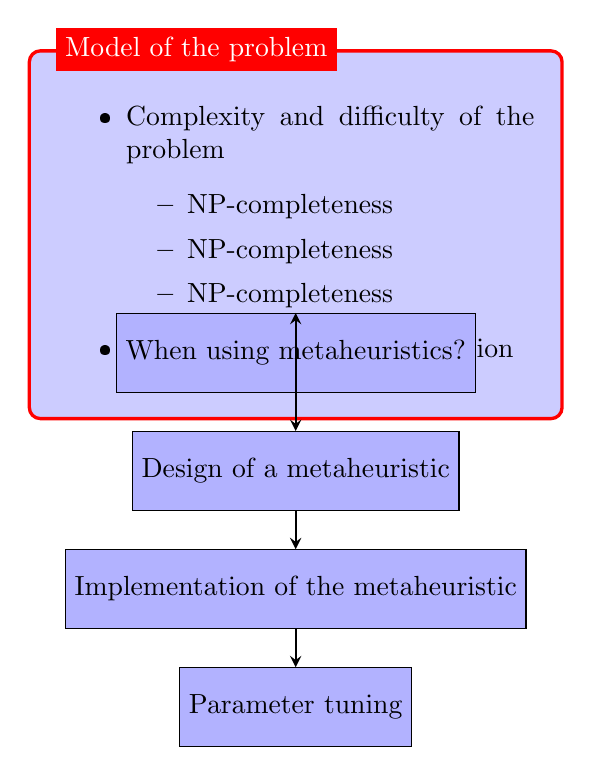
\begin{tikzpicture}[node distance=0.5cm][!h]
\centering
\node (pro1) [mybox] {
	\begin{minipage}{0.50\textwidth}
		 \begin{itemize}
		 	\item{Complexity and difficulty of the problem}
			\begin{itemize}
				\item{NP-completeness}
				\item{NP-completeness}
				\item{NP-completeness}
			\end{itemize}	
			\item{Requirements of the application}
		 \end{itemize}
		 
	\end{minipage}
};
\node[fancytitle, right=10pt] at (pro1.north west) {Model of the problem};

\node (pro2) [process, below of=pro1, yshift=-1.0cm] {When using metaheuristics?};
\node (pro3) [process, below of=pro2, yshift=-1.0cm] {Design of a metaheuristic};
\node (pro4) [process, below of=pro3, yshift=-1.0cm] {Implementation of the metaheuristic};
\node (pro5) [process, below of=pro4, yshift=-1.0cm] {Parameter tuning}; 


\draw [arrow] (pro1) -- (pro2);
\draw [arrow] (pro2) -- (pro3);
\draw [arrow] (pro3) -- (pro4);
\draw [arrow] (pro4) -- (pro5);

\end{tikzpicture}
\caption{Guidelines for solving SCP.}\label{fig:GuideSolvingSCP}
\end{figure}

\subsection{Main goal}
Solving the SCP using the Binary Global-Best HS metaheuristic algorithm.

\subsection{Specific objectives}
\begin{itemize}
\item Solve the SCP with the BGBHS metaheuristic and compare the results with benchmark of Beasley	\cite{citeulike:921349}	
%Solve the SCP with the HS metaheuristic and compare the results of unicost SCP using the same technique
\item Introduce new operators that make the results more close to the global optimum.
\item Search nearest optimal solutions to problems in the SCP.
\item Compare and analyze the results using different resolution strategies.
\end{itemize}





  \newpage
  
  \section{Theoretical Framework}\label{sec:marcoTeorico}
  Optimization problems are encountered in many domains: BigData, engineering, logistics, and business. An optimization problem may be defined by the couple $(S, f )$, where $S$ represents the set of feasible solutions, and $f : S \implies {\rm I\!R}$ the objective function to optimize. The objective function assigns to every solution
$s \in S$ of the search space a real number indicating its worth. The objective function
$f$ allows to define a total order relation between any pair of solutions in the search
space.\\
The global optimum is defined as  a solution $s^* \in S$ and it has a better objective function than all solutions of the search space, that is, $\forall  s \in  S$, $f(s^*) 	\leq f(s)$.

%Definici�n y clasificaci�n y conceptos asociados a la MH
\subsection{Metaheuristics and their classifications }
The $meta$ and $heuristic$ are Greek words, $meta$ it means $higher level$ and $heuristics$ means $to$ $find$, $to$ $know$ or $to$ $discover$. Metaheuristics are a set of intelligent strategies to enhance the efficiency of heuristic procedures.\\
A metaheuristic will be successful on a given optimizaction problem if it can provide a balance between exploration and exploitation. Exploration means to generate diverse solutions, associating them to different points of the search space on the global scale, while exploitation means to search in a local region by exploiting the information that a current good solution has been found in this region.
Exploration is often directed by use of randomization, which enables an algorithm to have the ability to jump between different bounded spaces and gives to the algorithm the capability to search optimal solutions globally.\\

The different metaheuristic approaches can be characterized by different aspects concerning the search path they follow or how search space is exploited \cite{citeulike:1859945}. The majority of these algorithms has a stochastic behavior and mimics biological or  physical processes. This presented classification was proposed by Beheshti et al. \cite{Beheshti:2014:CCA:2563733.2564085}, and can be understood better as shown in the (Figure \ref{fig:classification-of-mh}).

\squeezeup
\begin{figure}[ht] %ht
	\centering
  \includegraphics[width=0.70\textwidth]{MarcoTeorico/imagenes/classification_mh.png}
	\caption{Classification of metaheuristic}\label{fig:classification-of-mh}
\end{figure}
\squeezeup


~\\
\textbf{Nature-inspired vs. non-nature inspiration }
This class is based on the origin of algorithm. The majority of meta-heuristics are nature-inspired algorithms such as Black Hole (BH) \cite{Rubio2016}, Particle Swarm Optimization (PSO) \cite{Duran:2010:CPS:1645454.1645859} and Genetic Algorithms (GA) \cite{DBLP:conf/icsi/CrawfordSPJPO14}. Also, some of them are non-nature-inspired algorithms like Iterated Local Search (ILS) \cite{DBLP:journals/networks/AringhieriGHS16} and TabuSearch (TS) \cite{DBLP:journals/eswa/SotoCGMP13}.

~\\
\textbf{Population-based vs. single-point search}
There is a certain group of metaheuristics, that can be classified by the number of solutions in their lifecycle or execution, such as Trajectory methods, which are algorithms working based on a single solution at any time (Figure \ref{fig:trajectory-method}). On the other hand, Population-based algorithms perform searches with multiple initial points in a parallel style. Examples of these metaheuristics can be: Harmony Search (HS) \cite{DBLP:conf/ccece/Al-AjmiE14}, GA \cite{Aupetit2008} and PSO. 

\squeezeup
\begin{figure}[ht]
	\centering
  \includegraphics[width=0.4\textwidth]{MarcoTeorico/imagenes/trajectory-mh.png}
	\caption{Trajectory-based method}\label{fig:trajectory-method}
\end{figure}
\squeezeup

~\\
\textbf{Dynamic vs. static objective function}
Another way of classifying metaheuristics, is by the way of utilizing the objective function. Some algorithms maintain the objective function intact throughout the execution cycle, while others modify the objective function according to information collected at runtime.\\
An example of the second case presented, is Guided Local Search (GLS) \cite{DBLP:journals/eor/VansteenwegenSBO09}.  The idea behind this approach is to escape from local optima by changing the search landscape. 

~\\
\textbf{One vs. various neighborhood structures}
The majority of metaheuristic algorithms apply one single neighborhood structure. The fitness landscape topology remain unaltered thru the course of the algorithm while others, like Variable Neighborhood Search (VNS) \cite{DBLP:journals/anor/SarasolaDSA16}, employ a set of neighborhood structures. This latter structure gives the possibility to diversify the search by swapping between different fitness landscapes.

~\\
\textbf{Memory usage vs. memoryless methods}
One of the most interesting variables to classify a metaheuristic is undoubtedly use of memory. Short term usually is different from long term memory. The first kind usually keeps track of recently performed moves, or taken decisions. The second is usually an accumulation of synthetic parameters about the search. 

\subsection{Development Framework}
In an effort to maintain consistency in the structure of the proposed metaheuristic development, a well-defined model is followed, in order to structure the development steps of the proposed technique (Figure \ref{fig:GuideSolvingSCP}). \\
~\\
At first step, the problem is modeled and, based on its properties, application requirements are defined. In the particular case of this investigation the SCP is defined and validated against instances of benchmarck. The number of iterations has been considered, but runtime has not.\\

The second step basically corresponds to design the metaheuristic. In the case of this research, problems will be treated with variants of Harmony Search. That is to say not designed from the ground up, but certain elements are incorporated to improve the algorithm standard behavior. These elements are selected once known the nature of the problem to be solved and the metaheuristic to be used. Elements like the objective function to use and classification (Population based) are set by default.\\

The third step is to adopt a strategy of development of the technique or metaheuristic. In this research, it has been chosen to develop metaheruistics from scratch, thereby achieving maximum control of it. It was used for this purpose Python 2.7 as programming language and  PyCharm as IDE.\\

The fourth step is handling optimization parameters. There are two types of parameter tuning: Online and Off line. In this research, management of both types is performed to achieve good results. Specifically improving the metaheuristic proposal is based on the dynamic variation of the parameter that generates solutions. The following sections will go into detail on this subject.\\

The fifth and final step is to design experiments, get results and compare improvements. Then perform changes in parameters or operators so as to keep improving convergence, achieving an optimum balance between exploration and exploitation. This framework adopts an iterative approach because when step five is completed, systems can return to step one, two or three to seek a better solution.
%Definici�n formal / matem�tica del SCP y un ejemplo de soluci�n
\subsection{Set Covering Problem}
\subsubsection{SCP formulation}
The SCP is a well-known mathematical problem, which tries to cover a set of needs at the lowest possible cost. The SCP was included in the list of 21  $\mathcal{N} \mathcal{P}$-\textit{complet} problems of Karp \cite{DBLP:books/daglib/p/Karp10}. There are many practical uses for this problem, such as: crew scheduling \cite{ref02, ref08}, location of emergency facilities \cite{ref51,Vasko198485}, production planning in industry \cite{Vasko:1987:OSI:40299.40301,ref48, ref50}, vehicle routing \cite{ref07, ref27}, ship scheduling \cite{ref26, ref13}, network attack or defense \cite{ref14}, assembly line balancing \cite{ref28, ref41}, traffic assignment in satellite communication systems \cite{ref37, ceriaetal1998}, simplifying boolean expressions \cite{ref16}, the calculation of bounds in integer programs \cite{ref18}, information retrieval \cite{ref20}, political districting \cite{ref29}, crew scheduling problems in airlines \cite{doi:10.1287/inte.27.5.68}, among others.
The SCP can be formulated as follows:

\begin{equation} \label{ec:set-covering-1}  
\mbox{Minimize} \quad Z = \sum_{j = 1}^{n} c_j x_j
\end{equation}
Subject to:
\begin{equation} \label{ec:set-covering-2} 
\sum_{j = 1}^{n} a_{ij} x_j \geq 1 \quad  \forall i \in I
\end{equation}
\begin{equation} \label{ec:set-covering-3} 
x_j \in \{0,1\} \quad  \forall j \in J 
\end{equation}	

~\\
Let $A = (a_{ij})$ be a $m \times n$ 0-1 matrix with $I = \{ 1,\dots, m\}$ and $J = \{ 1,\dots, n\}$ be the row and column sets respectively. We say that column $j$ can be cover a row $i$ if $a_{ij} = 1$. Where $c_j$ is a nonnegative value that represents the cost of selecting the column $j$ and $x_j$ is a decision variable, it can be 1 if column $j$ is selected or 0 otherwise. The objective is to find a minimum cost subset $S \subseteq J$, such that each row $i \in I$ is covered by at least one column $j \in S$. In the following section, we present a simple way to understand the SCP, through an example.

\subsubsection{SCP sample solution}
Imagine that an ambulance station can meet the needs of an geographic zone. Similarly the ambulance station can cover all the needs of the nearby areas. For example, if a station is built in Zone 1 (Figure~\ref{fig:SetCovering}) ambulance station can meet the needs of neighboring areas, that is, it could also cover: Zone 1, Zone 2, Zone 3 and Zone 4.  This can be appreciated in equation (\ref{ec:rest1}).

In this example, we must fulfill the need to cover the geographical areas defined in accordance with the restrictions.

The restriction of this case is that all areas must be covered by at least one ambulance station and the goal is to minimize the number of stations built, the cost of building a station is the same for all areas. The $x_j$ variable represents the area $j$ which is $1$ if the ambulance station is built, and will be $0$ if not. As above, it can be formulated as follows:

\squeezeup
\begin{figure}[!http]
	\begin{center}
		\includegraphics[scale=0.25]{Introduccion/imagenes/SetCovering.png} %width=0.5\linewidth 
		\caption{Set Covering Problem example.}\label{fig:SetCovering}
	\end{center}
\end{figure}
\squeezeup


\scriptsize
\begin{equation} \label{ec:SetCoveringExample} 
\mbox{Min} \quad c_{1}x_{1} + c_{2}x_{2} + c_{3}x_{3} + c_{4}x_{4} + c_{5}x_{5} + c_{6}x_{6} + c_{7}x_{7} + c_{8}x_{8} + c_{9}x_{9} + c_{10}x_{10} + c_{11}x_{11}
\end{equation}

Subject to:
\begin{align}
x_{1} & + & x_{2} & + & x_{3} & + & x_{4} &  &  &  &  &  &  &  &  &  &  &  &  &  &  & \geq  1 \label{ec:rest1}  \\
x_{1} & + & x_{2} & + & x_{3} &  &  & + & x_{5} &  &  &  &  &  &  &  &  &  &  &  &  & \geq  1 \\
x_{1} & + & x_{2} & + & x_{3} & + & x_{4} & + & x_{5} & + & x_{6} &  &  &  &  &  &  &  &  &  &  & \geq  1 \\
x_{1} &  &  & + & x_{3} & + & x_{4} &  &  & + & x_{6} & + & x_{7} &  &  &  &  &  &  &  &  & \geq  1 \\
& & x_{2} & + & x_{3} &  &  & + & x_{5} & + & x_{6} &  &  & + & x_{8} & + & x_{9} &  &  &  &  & \geq  1 \\
& & & & x_{3} & + & x_{4} & + & x_{5} & + & x_{6} & + & x_{7} & + & x_{8} &  &  &  &  &  &  & \geq  1 \\
& & & & & & x_{4} & & & + & x_{6} & + & x_{7} & + & x_{8} & & & & & & & \geq  1 \\
& & & & & & & & x_{5} & + & x_{6} & + & x_{7} & + & x_{8} & + & x_{9} & + & x_{10} & & & \geq  1 \\
& & & & & & & & x_{5} & & & & & + & x_{8} & + & x_{9} & + & x_{10} & + & x_{11} & \geq  1 \\
& & & & & & & & & & & & & & x_{8} & + & x_{9} & + & x_{10} & + & x_{11} & \geq  1 \\
& & & & & & & & & & & & & & & & x_{9} & + & x_{10} & + & x_{11} & \geq  1 
\end{align}
\normalsize

The first constraint (\ref{ec:rest1}) indicates that to cover zone 1, it is possible to locate a station in the same area or in the border. The following restriction is for zone 2 and so on. One possible optimal solution for this problem is to locate ambulance stations in zones 3, 8 and 9. That is, $x_{3} = x_8 = x_9 = 1$ y $x_{1} = x_{2} = x_{4} = x_{5} = x_{6} = x_{7} = x_{10} = x_{11} = 0$. As shown in (Figure~\ref{fig:SetCovering2}).\\

\squeezeup
\begin{figure}[]%!http
	\begin{center}
		\includegraphics[scale=0.25]{Introduccion/imagenes/SetCoveringSolved.png}%width=0.5\linewidth
		\caption{Set Covering Problem solution.}\label{fig:SetCovering2}
	\end{center}	
\end{figure}
\squeezeup

The author propose solve the SCP, with a variation metaheuristic Harmony Search (HS) called Binary Global-Best Harmony Search to obtain satisfactory solutions within a reasonable time. HS mimics the process of musical improvisation, where musicians make adjustments in tone to achieve aesthetic harmony.
%Diagrama de trabajo
\squeezeup
\begin{figure}[H]
\centering
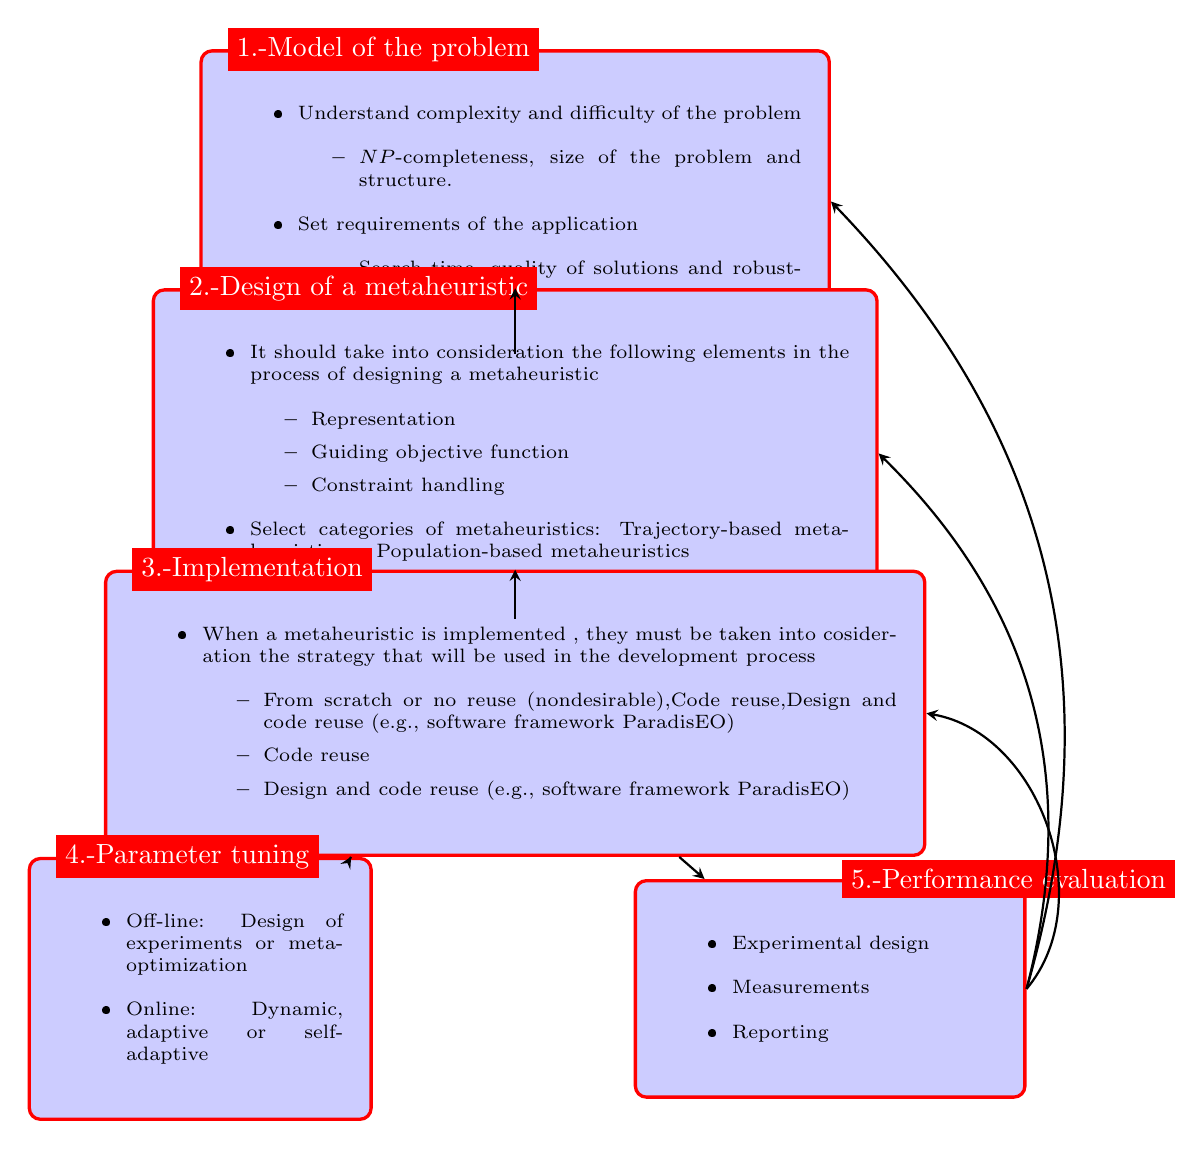
\begin{tikzpicture}[]

%==============================================
%Grafico de framework de trabajo 
%==============================================
%Nodo 1==============================================
\node (pro1) [mybox] {
	\begin{minipage}{0.60\textwidth}
	\scriptsize
		 \begin{itemize}
		 	\item{Understand complexity and difficulty of the problem}
			\begin{itemize}
				\item{$NP$-completeness, size of the problem and structure.}
			\end{itemize}	
			\item{Set requirements of the application}
			\begin{itemize}
				\item{Search time, quality of solutions and robustness.}
			\end{itemize}	
		 \end{itemize}
		 
	\end{minipage}
};
\node[fancytitle, right=10pt] at (pro1.north west) {1.-Model of the problem};

%Nodo 2==============================================
\node (pro2) [mybox, below of=pro1, yshift=-2.2cm] {
	\begin{minipage}{0.70\textwidth}
		\scriptsize
		 \begin{itemize}
		 	\item{It should take into consideration the following elements in the process of designing a metaheuristic}
			\begin{itemize}
				\item{Representation}
				\item{Guiding objective function}
				\item{Constraint handling}
			\end{itemize}
			\item{Select categories of metaheuristics: Trajectory-based metaheuristics or Population-based metaheuristics}
		 \end{itemize}
		 
	\end{minipage}
};
\node[fancytitle, right=10pt] at (pro2.north west) {2.-Design of a metaheuristic};

%Nodo 3============================================
\node (pro3) [mybox, below of=pro2, yshift=-2.3cm] {
	\begin{minipage}{0.80\textwidth}
		\scriptsize
		 \begin{itemize}
		 \item{When a metaheuristic is implemented , they must be taken into cosideration the strategy that will be used in the development process}
		 \begin{itemize}
		 	\item{From scratch or no reuse (nondesirable),Code reuse,Design and code reuse (e.g., software framework ParadisEO)}
			\item{Code reuse}
			\item{Design and code reuse (e.g., software framework ParadisEO)}
		 \end{itemize}
		\end{itemize}
	\end{minipage}
};
\node[fancytitle, right=10pt] at (pro3.north west) {3.-Implementation};

%Nodo 4=============================================
\node (pro4) [mybox,below of=pro3, yshift=-2.5cm, xshift=-4.0cm] {
	\begin{minipage}{0.30\textwidth}
		\scriptsize
		 \begin{itemize}
		 	\item{Off-line: Design of experiments or meta-optimization}
		 	\item{Online: Dynamic, adaptive or self-adaptive}
		 \end{itemize}
		 
	\end{minipage}
}; 
\node[fancytitle, right=10pt] at (pro4.north west) {4.-Parameter tuning};

%Nodo 5==============================================
\node (pro5) [mybox,below of=pro3, yshift=-2.5cm, xshift=4.0cm] {
	\begin{minipage}{0.35\textwidth}
		\scriptsize
		 \begin{itemize}
		 	\item{Experimental design}
			\item{Measurements}
			\item{Reporting}
		 \end{itemize}
		 
	\end{minipage}
}; 
\node[fancytitle, right=75pt] at (pro5.north west) {5.-Performance evaluation};
%==============================================
\draw [arrow] (pro1) --  (pro2);
\draw [arrow] (pro2) -- (pro3);
\draw [arrow] (pro3) -- (pro4);
\draw [arrow] (pro3) -- (pro5);
\draw [arrow] (pro5.east) to [bend right=30] (pro1.east);
\draw [arrow] (pro5.east) to [bend right=30] (pro2.east);
\draw [arrow] (pro5.east) to [bend right=60] (pro3.east);
\end{tikzpicture}
\caption{Guidelines for solving SCP.}\label{fig:GuideSolvingSCP}
\end{figure}
\squeezeup

\subsection{Harmony Search Metaheuristic}
Harmony Search (HS) is a population-based metaheuristic algorithm inspired from the musical process of searching for a perfect state of Harmony or Aesthetic Quality of a Harmony (AQH). The HS was proposed by Z. W. Geem et al.\cite{DBLP:journals/simulation/GeemKL01}. In other words, the main idea of the HS metaheuristic is to mimic the process performed by musicians when they try to play a beautiful harmony.

For the purpose of properly understand what is looking like a good solution in this metaheuristic, we must know the meaning of AQH. The AQH in an instrument it is essentially determined by its pitch (or frequency), sound quality, and amplitude (or loudness). The sound quality is mainly determined by the harmonic content that is in turn determined by the waveforms or modulations of the sound signal. However, the harmonics that it can generate will largely depend on the pitch or frequency range of the particular instrument \cite{Geem:2009:MHS:1643438}. Different notes have different frequencies. For example, the note A  has a fundamental frequency $f_0=440 Hz$. The fundamental frequency of each note can be seen in (Table~\ref{fig:musical_notes}). 

\begin{table}[H]
\centering
\begin{tabular}{|l|l|}
\hline
\textbf{Musical Note} & \textbf{Frequency} \\ \hline
C                     & 261,625565 Hz      \\ \hline
D                     & 293,664768 Hz      \\ \hline
E                     & 329,627557 Hz      \\ \hline
F                     & 349,228231 Hz      \\ \hline
G                     & 391,995436 Hz      \\ \hline
A                     & 440,000000 Hz      \\ \hline
B                     & 493,883301 Hz      \\ \hline
\end{tabular}
\caption{HS - Musical Notes}\label{fig:musical_notes}
\end{table}

Given the above, it is established that a good harmony has good AQH. The pitch of each musical instrument determines the AQH, just as the fitness function values determines the quality of solution.

In the music improvisation process, all musicians sound pitches within possible range together to make one harmony, If all pitches make a good harmony, each musician stores in his memory that experience and possibility of making a good harmony in increased next time. The same thing in optimization, the initial solution is generated randomly from decision variables within the possible range, If the objetive function values of these decision variables is good to make promising solution, then the possibility to make a good solution is increased next time.

In this document, the researcher set its focus on studying the classical SCP problem, given by equation \eqref{ec:set-covering-1}, where we want minimize the cost of solution.\\

The traditional HS metaheuristic has 4 steps, they will be reviewed in detail and then will be proposed the change to the original metaheuristic.\\ \\

\textbf{Step 1:  Initialize the problem and algorithm parameters.} \\
The optimization problem is defined as show in equation \eqref{ec:set-covering-1} where the goal is minimize $Z$ subjecto to \eqref{ec:set-covering-2} and \eqref{ec:set-covering-3}
The parameters required to solve the optimization problem are specified in this step, an initial HM is filled with a population of  Harmony Memory Size (HMS), harmonies are generated randomly.\\ 
In addition, the parameters of HS, that is, Harmony Memory Consideration Rate (HMCR) which determines the rate of selecting the value from the memory and Pitch Adjusting Rate (PAR) determines the probability of local improvement and number of improvisations (NI) are given when the metaheuristic begins.\\ \\
\textbf{Step 2: Initialize the harmony memory.} \\

\textbf{Step 3:  Improvise a new harmony.} \\

\textbf{Step 4: Update harmony memory.} \\
If the new generated harmony is better than the worst one in HM, then replace the worst harmony with the new one; otherwise, go to the next step. \\ \\
\textbf{Step 5: Check the stop criteria.} \\
If a stopping criterion is not satisfied, go to Step 2.

%TABLA (musician - > decision variables)
\squeezeup
\begin{table}[]
\centering
\begin{tabular}{|m{3.5cm}|m{8cm}|}
\hline
\includegraphics[width=30mm,scale=0.05]{MarcoTeorico/imagenes/musicos.png} & 
Each musician represents a decision variable,
according to the example shown, there would be 11 musicians, 	
since there are 11 decision variables $x_1\dots x_{11}$. \\ \hline
\end{tabular}
\caption{HS components - Musician}\label{fig:harmony_process_musician}
\end{table}
\squeezeup

%--VIOLIN (Instrument Pitch Range - > Range Value of decision variable)
\begin{table}[]
\centering
\begin{tabular}{|m{3.5cm}|m{8cm}|}
\hline
\includegraphics[width=15mm,scale=0.02]{MarcoTeorico/imagenes/violin.png} & The pitch range of the instrument represents the range of values that can take a decision variable. Given the nature of the problem, the possible values are ${\{0,1\}}$ \\  \hline\end{tabular}
\caption{HS components - Pitch range}\label{fig:harmony_process_pitch_range}
\end{table}


%--NOTA MUSICAL (Armonia -> Solucion)
\begin{table}[]
\centering
\begin{tabular}{|m{3.5cm}|m{8cm}|}
\hline
\includegraphics[width=15mm,scale=0.0005]{MarcoTeorico/imagenes/nota.png} & Musical harmony at a certain time, corresponds to a solution at a certain iteration.\\ \hline

\end{tabular}
\caption{HS components - Solution}\label{fig:harmony_process_solution}
\end{table}


% CALIDAD ESTETICA (Calidad de la armonia -> Calidad de la soluci�n)
\begin{table}[]
\centering
\begin{tabular}{|m{3.5cm}|m{8cm}|}
\hline
%$f=440\times2^{{(p_n-{69})}/12}$ & Aesthetics audience, judges whether harmony is good or not.� In the problem it refers to the objective function. \\ \hline

\includegraphics[width=30mm,scale=0.02]{MarcoTeorico/imagenes/audience.png} & Aesthetics audience, judges whether harmony is good or not.� In the problem it refers to the objective function.\\ \hline

\end{tabular}
\caption{HS components - Aesthetics audience}\label{fig:harmony_process_aesthetics}
\end{table}

%FIN TABLAS

\subsubsection{Global-Best Harmony Search Metaheuristic}
To further improve the convergence performance of HS and overcome some shortcomings of HS, a new variant of HS, called  Global-Best Harmony Search (GHS), was proposed by Omran and Mahdavi \cite{DBLP:journals/amc/OmranM08}. 
First, the GHS dynamically updates parameter PAR according to equation (\ref{ec:PAR-T}):

\begin{equation} \label{ec:PAR-T}
PAR(t) = PAR_{min}+\frac{PAR_{max} - PAR_{min}}{NI}t
\end{equation}

where $PAR(t)$ represents the pitch adjusting rate at generation $t$, $PAR_{min}$ and $PAR_{max}$  are the minimum and maximum adjusting rate, respectively.
The parameter $t$ is the iterative variable, and parameter $NI$ is the number of improvisations.


\subsubsection{Binary Global-Best Harmony Search Metaheuristic}

The HS is good at identifying the high performance regions of the solution space in a reasonable time, but poor at performing local search \cite{DBLP:journals/eswa/XiangALHZ14}. Namely, there is imbalance between the exploration and the exploitation of HS. Furthermore, HS designed for continuous space cannot be directly used to solve discrete combinatorial optimization problems.

In order to overcome the drawbacks of HS, a novel binary global-best harmony search (BGHS) is designed for binary optimization problems.

Owing to better performance of GHS, some modifications to GHS are introduced to further enhance the convergence performance of GHS. Then a novel binary coded GHS, a two-phase repair operator, and a greedy selection mechanism are integrated into the BGHS. And they are described in detail as follows.
























 [H]
  \newpage

  \section{Results}\label{sec:Resultados}
  The Table~\ref{table:results1} show the detailed results obtained by BGBHS. The second column $Z_{BKS}$ details the best known solution value of each instance evaluated. The next columns $Z_{MIN}$, $Z_{MAX}$, and $Z_{AVG}$ represents the minimum, maximum, and average objective function value respectively. The last column reports the relative percentage deviation (\textit{RPD}) value that represents the deviation of the objective value $Z$ (fitness) from $Z_{OPT}$ which in our case is the minimum value obtained for each instance. 

\begin{equation}\label{ec:RPD} 
\mbox{RPD} = \frac{100(Z_{MIN} - Z_{BKS})}{Z_{BKS}} 
\end{equation}
%!bp
\begin{table}[H]
	\scriptsize
	\begin{center}
		\resizebox*{1\textwidth}{!}{
		\begin{tabular*}{1\textwidth}{@{\extracolsep{\fill}} l l c c c c c c } 
			\hline
					&				&				&				&				&		\\
			Instance		&	$Z_{BKS}$	&	$Z_{MIN}$	&	$Z_{MAX}$	&	$Z_{AVG}$	&	RPD	\\
			
			%%%%%%%%%%%%%%
			\hline
			\hline
			   4.1 & 429 & 453 & 454 & 453.5 & 5.59& \\
                            4.2 & 512 & 561 & 563 & 562 & 9.57& \\
                            4.3 & 516 & 547 & 453 & 500 & 6.01& \\
                            4.4 & 494 & 537 & 548 & 542.5 & 8.7& \\
                            4.5 & 512 & 554 & 558 & 556 & 8.2& \\
                            4.6 & 560 & 612 & 708 & 660 & 9.29& \\
                            4.7 & 430 & 459 & 498 & 478.5 & 6.74& \\
                            4.8 & 492 & 526 & 725 & 625.5 & 6.91& \\
                            4.9 & 641 & 708 & 714 & 711 & 10.45& \\
                            4.10 & 514 & 586 & 597 & 591.5 & 14.01& \\
			   \hline
                            5.1 & 253 & 262 & 269 & 265.5 & 3.56& \\
                            5.2 & 302 & 328 & 345 & 336.5 & 8.61& \\
                            5.3 & 226 & 253 & 283 & 268 & 11.95& \\
                            5.4 & 242 & 278 & 293 & 285.5 & 14.88& \\
                            5.5 & 211 & 252 & 265 & 258.5 & 19.43& \\
                            5.6 & 213 & 286 & 342 & 314 & 34.27& \\
                            5.7 & 293 & 359 & 423 & 391 & 22.53& \\
                            5.8 & 288 & 436 & 529 & 482.5 & 51.39& \\
                            5.9 & 279 & 352 & 367 & 359.5 & 26.16& \\
                            5.10 & 265 & 303 & 321 & 312 & 14.34& \\
			   \hline
                            6.1 & 138 & 141 & 161 & 151 & 2.17& \\
                            6.2 & 146 & 157 & 175 & 166 & 7.53& \\
                            6.3 & 145 & 180 & 194 & 187 & 24.14& \\
                            6.4 & 131 & 159 & 163 & 161 & 21.37& \\
                            6.5 & 161 & 208 & 249 & 228.5 & 29.19& \\
			   \hline
                            A.1  & 253 & 280 & 299 & 289.5 & 10.67& \\
                            A.2  & 252 & 273 & 285 & 279 & 8.33& \\
                            A.3  & 232 & 274 & 286 & 280 & 18.1& \\
                            A.4  & 234 & 305 & 341 & 323 & 30.34& \\
                            A.5  & 236 & 261 & 273 & 267 & 10.59& \\
			   \hline
                            B.1  & 69 & 151 & 154 & 152.5 & 118.84& \\
                            B.2  & 76 & 157 & 169 & 163 & 106.58& \\
                            B.3  & 80 & 91 & 98 & 94.5 & 13.75& \\
                            B.4  & 79 & 167 & 192 & 179.5 & 111.39& \\
                            B.5  & 72 & 87 & 93 & 90 & 20.83& \\
			   \hline
                            C.1  & 227 & 270 & 281 & 275.5 & 18.94& \\
                            C.2  & 219 & 262 & 270 & 266 & 19.63& \\
                            C.3  & 243 & 349 & 351 & 350 & 43.62& \\
                            C.4  & 219 & 275 & 282 & 278.5 & 25.57& \\
                            C.5  & 215 & 244 & 255 & 249.5 & 13.49& \\
			   \hline
                            D.1  & 60 & 111 & 123 & 117 & 85& \\
                            D.2  & 66 & 79 & 84 & 81.5 & 19.7& \\
                            D.3  & 72 & 100 & 193 & 146.5 & 38.89& \\
                            D.4  & 62 & 104 & 109 & 106.5 & 67.74& \\
                            D.5  & 61 & 133 & 142 & 137.5 & 118.03& \\
			\hline
			%%%%%%%%%%%%%%
		\end{tabular*}
		}
	\end{center}
	\caption{Experimental results of SCP benchmarks (4, 5, 6, A, B, C and D sets).}\label{table:results1}
\end{table}










\begin{table}[H]
	\scriptsize
	\begin{center}
		\resizebox*{1\textwidth}{!}{
		\begin{tabular*}{1\textwidth}{@{\extracolsep{\fill}} l l c c c c c c } 
			\hline
					&				&				&				&				&		\\
			Instance		&	$Z_{BKS}$	&	$Z_{MIN}$	&	$Z_{MAX}$	&	$Z_{AVG}$	&	RPD	\\
			
			%%%%%%%%%%%%%%
			\hline
			\hline
			   4.1 & 429 & 430 & 520 & 475 & 0.23& \\
                            4.2 & 512 & 516 & 537 & 526.5 & 0.78& \\
                            4.3 & 516 & 520 & 532 & 526 & 0.78& \\
                            4.4 & 494 & 512 & 520 & 516 & 3.64& \\
                            4.5 & 512 & 519 & 583 & 551 & 1.37& \\
                            4.6 & 560 & 568 & 440 & 504 & 1.43& \\
                            4.7 & 430 & 432 & 512 & 472 & 0.47& \\
                            4.8 & 492 & 497 & 952 & 724.5 & 1.02& \\
                            4.9 & 641 & 643 & 809 & 726 & 0.31& \\
                            4.10 & 514 & 520 & 280 & 400 & 1.17& \\
			   \hline
                            5.1 & 253 & 255 & 393 & 324 & 0.79& \\
                            5.2 & 302 & 303 & 239 & 271 & 0.33& \\
                            5.3 & 226 & 242 & 255 & 248.5 & 7.08& \\
                            5.4 & 242 & 244 & 220 & 232 & 0.83& \\
                            5.5 & 211 & 213 & 215 & 214 & 0.95& \\
                            5.6 & 213 & 223 & 311 & 267 & 4.69& \\
                            5.7 & 293 & 299 & 299 & 299 & 2.05& \\
                            5.8 & 288 & 300 & 295 & 297.5 & 4.17& \\
                            5.9 & 279 & 282 & 280 & 281 & 1.08& \\
                            5.10 & 265 & 271 & 272 & 271.5 & 2.26& \\
			   \hline
                            6.1 & 138 & 140 & 226 & 183 & 1.45& \\
                            6.2 & 146 & 147 & 248 & 197.5 & 0.68& \\
                            6.3 & 145 & 149 & 153 & 151 & 2.76& \\
                            6.4 & 131 & 133 & 172 & 152.5 & 1.53& \\
                            6.5 & 161 & 163 & 280 & 221.5 & 1.24& \\
			   \hline
                            A.1  & 253 & 270 & 300 & 285 & 6.72& \\
                            A.2  & 252 & 260 & 302 & 281 & 3.17& \\
                            A.3  & 232 & 241 & 329 & 285 & 3.88& \\
                            A.4  & 234 & 250 & 258 & 254 & 6.84& \\
                            A.5  & 236 & 242 & 90 & 166 & 2.54& \\
			   \hline
                            B.1  & 69 & 76 & 120 & 98 & 10.14& \\
                            B.2  & 76 & 80 & 97 & 88.5 & 5.26& \\
                            B.3  & 80 & 88 & 84 & 86 & 10& \\
                            B.4  & 79 & 81 & 92 & 86.5 & 2.53& \\
                            B.5  & 72 & 74 & 400 & 237 & 2.78& \\
			   \hline
                            C.1  & 227 & 235 & 420 & 327.5 & 3.52& \\
                            C.2  & 219 & 254 & 399 & 326.5 & 15.98& \\
                            C.3  & 243 & 246 & 528 & 387 & 1.23& \\
                            C.4  & 219 & 225 & 623 & 424 & 2.74& \\
                            C.5  & 215 & 222 & 400 & 311 & 3.26& \\
			   \hline
                            D.1  & 60 & 67 & 420 & 243.5 & 11.67& \\
                            D.2  & 66 & 69 & 399 & 234 & 4.55& \\
                            D.3  & 72 & 85 & 528 & 306.5 & 18.06& \\
                            D.4  & 62 & 66 & 623 & 344.5 & 6.45& \\
                            D.5  & 61 & 71 & 87 & 79 & 16.39& \\
			\hline
			%%%%%%%%%%%%%%
		\end{tabular*}
		}
	\end{center}
	\caption{Experimental results of SCP benchmarks (4, 5, 6, A, B, C and D sets) With variable $p$ parameter.}\label{table:results2}
\end{table}
  \newpage
  
  \section{Conclusion}\label{sec:Conclusi�n}
  In this chapter, a general conclusion of the work will be addressed, starting from the basis of the exhaustive detail seen in chapter \ref{sec:Analisys}.
We will then move on to a view of the overall results compared to other metaheuristics. Finally, we will make an approach that lay the foundation for future work.

\subsection{Global analysis}
This work began with the need to obtain a thorough knowledge of metaheuristics, with the ultimate aim of getting into the world of information security and to be able to apply this method in it. In order to achieve this goal the first thing was to know in depth how a metaheuristic worked, for it was studied in detail the behavior of several algorithms
To find one that met certain characteristics that made it interesting to study. In this case, Harmony Search was selected.\\

Once the algorithm or metaheuristic was selected the next step was to confront the decision to choose a type problem, to which to apply the metaheuristic and to look for possible solutions. According to what was reviewed in different publications, SCP was chosen because it had broad applications and was easy to implement.\\

After having selected Harmony Search and SCP, it is necessary to review the behavior against other metaheuristics, for which it is necessary to use a set of known data, for which we use the library of Beasley\\

After specifying the above, we evaluated the behavior of the selected metaheuristics BGBHS, compared to others with similar characteristics. As you can see in the analysis and results section. The selected metaheuristic presents poor performance in relation to Black Hole S-Shape and Improved Black Hole, according to RPD measurements.\\

Considering the comparative results of the RPDs obtained, the need to improve BGBHS was presented, for which a novel method is proposed that aims to achieve a wider variation in the initial population of solutions, thus obtaining a better convergence, but Mainly a better exploration since the solutions depart being feasible but little optimum then vary until they are feasible and close to the optimum.\\
  \newpage

  \section{Appendix}\label{sec:Anexo}
  
%Instancia 4
\subsection{Instance 4.1}


\begin{table}[H]
\centering
\begin{tabular}{ | l | l | l | l | l | l | }
\hline
	Method & Optimum & Min & Max & Avg & RPD \\ \hline
	BGBHS & 429 & 534 &  &  & 24.475524475524477 \\ \hline
	BGBHS & 429 & 553 &  &  & 28.904428904428904 \\ \hline
	BGBHS & 429 & 533 &  &  & 24.242424242424242 \\ \hline
	BGBHS & 429 & 600 &  &  & 39.86013986013986 \\ \hline
	BGBHS & 429 & 438 &  &  & 2.0979020979020979 \\ \hline
	BGBHS & 429 & 460 &  &  & 7.2261072261072261 \\ \hline
	BGBHS & 429 & 455 &  &  & 6.0606060606060606 \\ \hline
	BGBHS & 429 & 470 &  &  & 9.5571095571095572 \\ \hline
	BGBHS & 429 & 533 &  &  & 24.242424242424242 \\ \hline
	BGBHS & 429 & 532 &  &  & 24.009324009324008 \\ \hline
	BGBHS IMPROVED & 429 & 451 &  &  & 5.1282051282051286 \\ \hline
	BGBHS IMPROVED & 429 & 440 &  &  & 2.5641025641025643 \\ \hline
	BGBHS IMPROVED & 429 & 460 &  &  & 7.2261072261072261 \\ \hline
	BGBHS IMPROVED & 429 & 445 &  &  & 3.7296037296037294 \\ \hline
	BGBHS IMPROVED & 429 & 470 &  &  & 9.5571095571095572 \\ \hline
	BGBHS IMPROVED & 429 & 430 &  &  & 0.23310023310023309 \\ \hline
	BGBHS IMPROVED & 429 & 430 &  &  & 0.23310023310023309 \\ \hline
	BGBHS IMPROVED & 429 & 432 &  &  & 0.69930069930069927 \\ \hline
	BGBHS IMPROVED & 429 & 435 &  &  & 1.3986013986013985 \\ \hline
	BGBHS IMPROVED & 429 & 430 &  &  & 0.23310023310023309 \\ \hline
\end{tabular}

\caption{Instance 4.1}
\label{tblscp41}
\end{table}



\newpage
\subsection{Instance 4.2}

\begin{table}[H]
\centering
\begin{tabular}{ | l | l | l | l | l | l | }
\hline
	Method & Optimum & Min & Max & Avg & RPD \\ \hline
	BGBHS & 512 & 632 &  &  & 23.4375 \\ \hline
	BGBHS & 512 & 662 &  &  & 29.296875 \\ \hline
	BGBHS & 512 & 660 &  &  & 28.90625 \\ \hline
	BGBHS & 512 & 602 &  &  & 17.578125 \\ \hline
	BGBHS & 512 & 641 &  &  & 25.1953125 \\ \hline
	BGBHS & 512 & 644 &  &  & 25.78125 \\ \hline
	BGBHS & 512 & 642 &  &  & 25.390625 \\ \hline
	BGBHS & 512 & 647 &  &  & 26.3671875 \\ \hline
	BGBHS & 512 & 641 &  &  & 25.1953125 \\ \hline
	BGBHS & 512 & 623 &  &  & 21.6796875 \\ \hline
	BGBHS IMPROVED & 512 & 550 &  &  & 7.421875 \\ \hline
	BGBHS IMPROVED & 512 & 560 &  &  & 9.375 \\ \hline
	BGBHS IMPROVED & 512 & 563 &  &  & 9.9609375 \\ \hline
	BGBHS IMPROVED & 512 & 520 &  &  & 1.5625 \\ \hline
	BGBHS IMPROVED & 512 & 523 &  &  & 2.1484375 \\ \hline
	BGBHS IMPROVED & 512 & 555 &  &  & 8.3984375 \\ \hline
	BGBHS IMPROVED & 512 & 524 &  &  & 2.34375 \\ \hline
	BGBHS IMPROVED & 512 & 518 &  &  & 1.171875 \\ \hline
	BGBHS IMPROVED & 512 & 519 &  &  & 1.3671875 \\ \hline
	BGBHS IMPROVED & 512 & 520 &  &  & 1.5625 \\ \hline
\end{tabular}
\caption{Instance 4.2}
\label{tblscp42}
\end{table}

\newpage
\subsection{Instance 4.3}
\begin{table}[H]
\centering
\begin{tabular}{ | l | l | l | l | l | l | }
\hline
	Method & Optimum & Min & Max & Avg & RPD \\ \hline
	BGBHS & 516 &  &  &  & -100 \\ \hline
	BGBHS & 516 &  &  &  & -100 \\ \hline
	BGBHS & 516 &  &  &  & -100 \\ \hline
	BGBHS & 516 &  &  &  & -100 \\ \hline
	BGBHS & 516 &  &  &  & -100 \\ \hline
	BGBHS & 516 &  &  &  & -100 \\ \hline
	BGBHS & 516 &  &  &  & -100 \\ \hline
	BGBHS & 516 &  &  &  & -100 \\ \hline
	BGBHS & 516 &  &  &  & -100 \\ \hline
	BGBHS & 516 &  &  &  & -100 \\ \hline
	BGBHS IMPROVED & 516 & 613 &  &  & 18.7984496124031 \\ \hline
	BGBHS IMPROVED & 516 &  &  &  & -100 \\ \hline
	BGBHS IMPROVED & 516 &  &  &  & -100 \\ \hline
	BGBHS IMPROVED & 516 &  &  &  & -100 \\ \hline
	BGBHS IMPROVED & 516 &  &  &  & -100 \\ \hline
	BGBHS IMPROVED & 516 &  &  &  & -100 \\ \hline
	BGBHS IMPROVED & 516 &  &  &  & -100 \\ \hline
	BGBHS IMPROVED & 516 &  &  &  & -100 \\ \hline
	BGBHS IMPROVED & 516 &  &  &  & -100 \\ \hline
	BGBHS IMPROVED & 516 &  &  &  & -100 \\ \hline
\end{tabular}

\caption{Instance 4.3}
\label{tblscp43}
\end{table}
\newpage

\subsection{Instance 4.4}
\begin{table}[H]
\centering
\begin{tabular}{ | l | l | l | l | l | l | }
\hline
	Method & Optimum & Min & Max & Avg & RPD \\ \hline
	BGBHS & 494 &  &  &  & -100 \\ \hline
	BGBHS & 494 &  &  &  & -100 \\ \hline
	BGBHS & 494 &  &  &  & -100 \\ \hline
	BGBHS & 494 &  &  &  & -100 \\ \hline
	BGBHS & 494 &  &  &  & -100 \\ \hline
	BGBHS & 494 &  &  &  & -100 \\ \hline
	BGBHS & 494 &  &  &  & -100 \\ \hline
	BGBHS & 494 &  &  &  & -100 \\ \hline
	BGBHS & 494 &  &  &  & -100 \\ \hline
	BGBHS & 494 &  &  &  & -100 \\ \hline
	BGBHS IMPROVED & 494 &  &  &  & -100 \\ \hline
	BGBHS IMPROVED & 494 &  &  &  & -100 \\ \hline
	BGBHS IMPROVED & 494 &  &  &  & -100 \\ \hline
	BGBHS IMPROVED & 494 &  &  &  & -100 \\ \hline
	BGBHS IMPROVED & 494 &  &  &  & -100 \\ \hline
	BGBHS IMPROVED & 494 &  &  &  & -100 \\ \hline
	BGBHS IMPROVED & 494 &  &  &  & -100 \\ \hline
	BGBHS IMPROVED & 494 &  &  &  & -100 \\ \hline
	BGBHS IMPROVED & 494 &  &  &  & -100 \\ \hline
	BGBHS IMPROVED & 494 &  &  &  & -100 \\ \hline
\end{tabular}

\caption{Instance 4.4}
\label{tblscp44}
\end{table}
\newpage

\subsection{Instance 4.5}
\begin{table}[H]
\centering
\begin{tabular}{ | l | l | l | l | l | l | }
\hline
	Method & Optimum & Min & Max & Avg & RPD \\ \hline
	BGBHS & 512 &  &  &  & -100 \\ \hline
	BGBHS & 512 &  &  &  & -100 \\ \hline
	BGBHS & 512 &  &  &  & -100 \\ \hline
	BGBHS & 512 &  &  &  & -100 \\ \hline
	BGBHS & 512 &  &  &  & -100 \\ \hline
	BGBHS & 512 &  &  &  & -100 \\ \hline
	BGBHS & 512 &  &  &  & -100 \\ \hline
	BGBHS & 512 &  &  &  & -100 \\ \hline
	BGBHS & 512 &  &  &  & -100 \\ \hline
	BGBHS & 512 &  &  &  & -100 \\ \hline
	BGBHS IMPROVED & 512 &  &  &  & -100 \\ \hline
	BGBHS IMPROVED & 512 &  &  &  & -100 \\ \hline
	BGBHS IMPROVED & 512 &  &  &  & -100 \\ \hline
	BGBHS IMPROVED & 512 &  &  &  & -100 \\ \hline
	BGBHS IMPROVED & 512 &  &  &  & -100 \\ \hline
	BGBHS IMPROVED & 512 &  &  &  & -100 \\ \hline
	BGBHS IMPROVED & 512 &  &  &  & -100 \\ \hline
	BGBHS IMPROVED & 512 &  &  &  & -100 \\ \hline
	BGBHS IMPROVED & 512 &  &  &  & -100 \\ \hline
	BGBHS IMPROVED & 512 &  &  &  & -100 \\ \hline
\end{tabular}

\caption{Instance 4.5}
\label{tblscp45}
\end{table}
\newpage

\subsection{Instance 4.6}
\begin{table}[H]
\centering
\begin{tabular}{ | l | l | l | l | l | l | }
\hline
	Method & Optimum & Min & Max & Avg & RPD \\ \hline
	BGBHS & 560 &  &  &  & -100 \\ \hline
	BGBHS & 560 &  &  &  & -100 \\ \hline
	BGBHS & 560 &  &  &  & -100 \\ \hline
	BGBHS & 560 &  &  &  & -100 \\ \hline
	BGBHS & 560 &  &  &  & -100 \\ \hline
	BGBHS & 560 &  &  &  & -100 \\ \hline
	BGBHS & 560 &  &  &  & -100 \\ \hline
	BGBHS & 560 &  &  &  & -100 \\ \hline
	BGBHS & 560 &  &  &  & -100 \\ \hline
	BGBHS & 560 &  &  &  & -100 \\ \hline
	BGBHS IMPROVED & 560 &  &  &  & -100 \\ \hline
	BGBHS IMPROVED & 560 &  &  &  & -100 \\ \hline
	BGBHS IMPROVED & 560 &  &  &  & -100 \\ \hline
	BGBHS IMPROVED & 560 &  &  &  & -100 \\ \hline
	BGBHS IMPROVED & 560 &  &  &  & -100 \\ \hline
	BGBHS IMPROVED & 560 &  &  &  & -100 \\ \hline
	BGBHS IMPROVED & 560 &  &  &  & -100 \\ \hline
	BGBHS IMPROVED & 560 &  &  &  & -100 \\ \hline
	BGBHS IMPROVED & 560 &  &  &  & -100 \\ \hline
	BGBHS IMPROVED & 560 &  &  &  & -100 \\ \hline
\end{tabular}

\caption{Instance 4.6}
\label{tblscp46}
\end{table}
\newpage

\subsection{Instance 4.7}
\begin{table}[H]
\centering
\begin{tabular}{ | l | l | l | l | l | l | }
\hline
	Method & Optimum & Min & Max & Avg & RPD \\ \hline
	BGBHS & 430 &  &  &  & -100 \\ \hline
	BGBHS & 430 &  &  &  & -100 \\ \hline
	BGBHS & 430 &  &  &  & -100 \\ \hline
	BGBHS & 430 &  &  &  & -100 \\ \hline
	BGBHS & 430 &  &  &  & -100 \\ \hline
	BGBHS & 430 &  &  &  & -100 \\ \hline
	BGBHS & 430 &  &  &  & -100 \\ \hline
	BGBHS & 430 &  &  &  & -100 \\ \hline
	BGBHS & 430 &  &  &  & -100 \\ \hline
	BGBHS & 430 &  &  &  & -100 \\ \hline
	BGBHS IMPROVED & 430 &  &  &  & -100 \\ \hline
	BGBHS IMPROVED & 430 &  &  &  & -100 \\ \hline
	BGBHS IMPROVED & 430 &  &  &  & -100 \\ \hline
	BGBHS IMPROVED & 430 &  &  &  & -100 \\ \hline
	BGBHS IMPROVED & 430 &  &  &  & -100 \\ \hline
	BGBHS IMPROVED & 430 &  &  &  & -100 \\ \hline
	BGBHS IMPROVED & 430 &  &  &  & -100 \\ \hline
	BGBHS IMPROVED & 430 &  &  &  & -100 \\ \hline
	BGBHS IMPROVED & 430 &  &  &  & -100 \\ \hline
	BGBHS IMPROVED & 430 &  &  &  & -100 \\ \hline
\end{tabular}

\caption{Instance 4.7}
\label{tblscp47}
\end{table}
\newpage

\subsection{Instance 4.8}
\begin{table}[H]
\centering
\begin{tabular}{ | l | l | l | l | l | l | }
\hline
	Method & Optimum & Min & Max & Avg & RPD \\ \hline
	BGBHS & 492 &  &  &  & -100 \\ \hline
	BGBHS & 492 &  &  &  & -100 \\ \hline
	BGBHS & 492 &  &  &  & -100 \\ \hline
	BGBHS & 492 &  &  &  & -100 \\ \hline
	BGBHS & 492 &  &  &  & -100 \\ \hline
	BGBHS & 492 &  &  &  & -100 \\ \hline
	BGBHS & 492 &  &  &  & -100 \\ \hline
	BGBHS & 492 &  &  &  & -100 \\ \hline
	BGBHS & 492 &  &  &  & -100 \\ \hline
	BGBHS & 492 &  &  &  & -100 \\ \hline
	BGBHS IMPROVED & 492 &  &  &  & -100 \\ \hline
	BGBHS IMPROVED & 492 &  &  &  & -100 \\ \hline
	BGBHS IMPROVED & 492 &  &  &  & -100 \\ \hline
	BGBHS IMPROVED & 492 &  &  &  & -100 \\ \hline
	BGBHS IMPROVED & 492 &  &  &  & -100 \\ \hline
	BGBHS IMPROVED & 492 &  &  &  & -100 \\ \hline
	BGBHS IMPROVED & 492 &  &  &  & -100 \\ \hline
	BGBHS IMPROVED & 492 &  &  &  & -100 \\ \hline
	BGBHS IMPROVED & 492 &  &  &  & -100 \\ \hline
	BGBHS IMPROVED & 492 &  &  &  & -100 \\ \hline
\end{tabular}

\caption{Instance 4.8}
\label{tblscp48}
\end{table}
\newpage

\subsection{Instance 4.9}
\begin{table}[H]
\centering
\begin{tabular}{ | l | l | l | l | l | l | }
\hline
	Method & Optimum & Min & Max & Avg & RPD \\ \hline
	BGBHS & 641 &  &  &  & -100 \\ \hline
	BGBHS & 641 &  &  &  & -100 \\ \hline
	BGBHS & 641 &  &  &  & -100 \\ \hline
	BGBHS & 641 &  &  &  & -100 \\ \hline
	BGBHS & 641 &  &  &  & -100 \\ \hline
	BGBHS & 641 &  &  &  & -100 \\ \hline
	BGBHS & 641 &  &  &  & -100 \\ \hline
	BGBHS & 641 &  &  &  & -100 \\ \hline
	BGBHS & 641 &  &  &  & -100 \\ \hline
	BGBHS & 641 &  &  &  & -100 \\ \hline
	BGBHS IMPROVED & 641 &  &  &  & -100 \\ \hline
	BGBHS IMPROVED & 641 &  &  &  & -100 \\ \hline
	BGBHS IMPROVED & 641 &  &  &  & -100 \\ \hline
	BGBHS IMPROVED & 641 &  &  &  & -100 \\ \hline
	BGBHS IMPROVED & 641 &  &  &  & -100 \\ \hline
	BGBHS IMPROVED & 641 &  &  &  & -100 \\ \hline
	BGBHS IMPROVED & 641 &  &  &  & -100 \\ \hline
	BGBHS IMPROVED & 641 &  &  &  & -100 \\ \hline
	BGBHS IMPROVED & 641 &  &  &  & -100 \\ \hline
	BGBHS IMPROVED & 641 &  &  &  & -100 \\ \hline
\end{tabular}

\caption{Instance 4.9}
\label{tblscp49}
\end{table}
\newpage

\subsection{Instance 4.10}
\begin{table}[H]
\centering

\caption{Instance 4.10}
\label{tblscp410}
\end{table}
\newpage

%Instancia 5
\subsection{Instance 5.1}
\begin{table}[H]
\centering

\caption{Instance 5.1}
\label{tblscp51}
\end{table}
\newpage

\subsection{Instance 5.2}
\begin{table}[H]
\centering

\caption{Instance 5.2}
\label{tblscp52}
\end{table}
\newpage

\subsection{Instance 5.3}
\begin{table}[H]
\centering

\caption{Instance 5.3}
\label{tblscp53}
\end{table}
\newpage

\subsection{Instance 5.4}
\begin{table}[H]
\centering

\caption{Instance 5.4}
\label{tblscp54}
\end{table}
\newpage

\subsection{Instance 5.5}
\begin{table}[H]
\centering

\caption{Instance 5.5}
\label{tblscp55}
\end{table}
\newpage

\subsection{Instance 5.6}
\begin{table}[H]
\centering

\caption{Instance 5.6}
\label{tblscp56}
\end{table}
\newpage

\subsection{Instance 5.7}
\begin{table}[H]
\centering

\caption{Instance 5.7}
\label{tblscp57}
\end{table}
\newpage

\subsection{Instance 5.8}
\begin{table}[H]
\centering

\caption{Instance 5.8}
\label{tblscp58}
\end{table}
\newpage

\subsection{Instance 5.9}
\begin{table}[H]
\centering

\caption{Instance 5.9}
\label{tblscp59}
\end{table}
\newpage

\subsection{Instance 5.10}
\begin{table}[H]
\centering

\caption{Instance 5.10}
\label{tblscp510}
\end{table}
\newpage


%Instancia 6
\subsection{Instance 6.1}
\begin{table}[H]
\centering

\caption{Instance 6.1}
\label{tblscp61}
\end{table}
\newpage

\subsection{Instance 6.2}
\begin{table}[H]
\centering

\caption{Instance 6.2}
\label{tblscp62}
\end{table}
\newpage

\subsection{Instance 6.3}
\begin{table}[H]
\centering

\caption{Instance 6.3}
\label{tblscp63}
\end{table}
\newpage

\subsection{Instance 6.4}
\begin{table}[H]
\centering

\caption{Instance 6.4}
\label{tblscp64}
\end{table}
\newpage

\subsection{Instance 6.5}
\begin{table}[H]
\centering

\caption{Instance 6.5}
\label{tblscp65}
\end{table}
\newpage

%Instancia A
\subsection{Instance A.1}
\begin{table}[H]
\centering

\caption{Instance A.1}
\label{tblscpA1}
\end{table}

\newpage

\subsection{Instance A.2}
\begin{table}[H]
\centering

\caption{Instance A.2}
\label{tblscpA2}
\end{table}

\newpage
\subsection{Instance A.3}
\begin{table}[H]
\centering

\caption{Instance A.3}
\label{tblscpA3}
\end{table}

\newpage
\subsection{Instance A.4}
\begin{table}[H]
\centering

\caption{Instance A.3}
\label{tblscpA3}
\end{table}

\newpage
\subsection{Instance A.5}
\begin{table}[H]
\centering

\caption{Instance A.5}
\label{tblscpA5}
\end{table}

\newpage

%Instancia B
\subsection{Instance B.1}
\begin{table}[H]
\centering

\caption{Instance B.1}
\label{tblscpB1}
\end{table}

\newpage
\subsection{Instance B.2}
\begin{table}[H]
\centering

\caption{Instance B.2}
\label{tblscpB2}
\end{table}
\newpage

\subsection{Instance B.3}
\begin{table}[H]
\centering

\caption{Instance B.3}
\label{tblscpB3}
\end{table}
\newpage

\subsection{Instance B.4}
\begin{table}[H]
\centering

\caption{Instance B.4}
\label{tblscpB4}
\end{table}
\newpage

\subsection{Instance B.5}
\begin{table}[H]
\centering

\caption{Instance B.5}
\label{tblscpB5}
\end{table}
\newpage

%Instancia C
\subsection{Instance C.1}
\begin{table}[H]
\centering

\caption{Instance C.1}
\label{tblscpC1}
\end{table}
\newpage
\subsection{Instance C.2}
\begin{table}[H]
\centering

\caption{Instance C.2}
\label{tblscpC2}
\end{table}
\newpage

\subsection{Instance C.3}
\begin{table}[H]
\centering

\caption{Instance C.3}
\label{tblscpC3}
\end{table}
\newpage

\subsection{Instance C.4}
\begin{table}[H]
\centering

\caption{Instance C.4}
\label{tblscpC4}
\end{table}
\newpage

\subsection{Instance C.5}
\begin{table}[H]
\centering

\caption{Instance C.5}
\label{tblscpC5}
\end{table}
\newpage

%Instancia D
\subsection{Instance D.1}
\begin{table}[H]
\centering

\caption{Instance D.1}
\label{tblscpD1}
\end{table}
\newpage

\subsection{Instance D.2}
\begin{table}[H]
\centering

\caption{Instance D.2}
\label{tblscpD2}
\end{table}
\newpage

\subsection{Instance D.3}
\begin{table}[H]
\centering

\caption{Instance D.3}
\label{tblscpD3}
\end{table}
\newpage

\subsection{Instance D.4}
\begin{table}[H]
\centering

\caption{Instance D.4}
\label{tblscpD4}
\end{table}
\newpage

\subsection{Instance D.5}
\begin{table}[H]
\centering

\caption{Instance D.5}
\label{tblscpD5}
\end{table}
\newpage



  \newpage
  
%%=============================================================================
%% Biblio
\bibliographystyle{ieeetr}
\bibliography{bibliography}	

\end{document}